% !TEX root = ../main.tex
\documentclass[../main.tex]{subfiles}
\begin{document}
В этой главе рассмотрены варианты локальных угломерных навигационных систем, которые позволяют определять координаты и угловую ориентацию подвижных объектов.

%
% TODO: Привести в соответствие с первой статьей
%
%
\subsection{Простейшая локальная навигационная система}
Пусть три радиоориентира расположены в точках $M_1\left(x_1, y_1, z_1\right)$, $M_2\left(x_2, y_2, z_2\right)$ и $M_3\left(x_3, y_3, z_3\right)$ с заданными координатами и находятся не на одной прямой, а ФЦ БПА, размещенной на подвижном объекте находится в точке $M_0\left(x, y, z\right)$. В таком случае, эти четыре точки образуют в пространстве треугольную пирамиду, схематическое представление которой приведено на рисунке \ref{fig:tetrahedron:pic1}. Обозначим через $\ell_i$ длину бокового ребра $M_0M_i$, через $d_{ij}$ "--- длину ребра основания $M_iM_j$, а через $\alpha_{ij}$ "--- плоский угол $\angle M_iM_0M_j$ при вершине пирамиды. Пространственное положение подвижного объекта и радиоориентиров также будем определять с помощью радиус-векторов $\mathbf{r}_0 = \left(x, y, z\right)$ и $\mathbf{r}_i = \left(x_i, y_i, z_i\right)$ соответственно.

\begin{figure}[htbp]
    \centering

    \fbox{\includegraphics[width=0.6\columnwidth]{3/tetrahedron/pic1}}

    \caption{Схема размещения в пространстве трех радиоориентиров и фазового центра БПА}
    \label{fig:tetrahedron:pic1}
\end{figure}

Допустим, что в результате азимутально-угломестного радиопеленгования радиоориентиров с использованием БПА определены три пары азимутов $\alpha_{i}$ и углов места $\varepsilon_{i}$. Тогда в связанной системе координат БПА можно определить три единичных вектора $\mathbf{s}_{\text{св}i}$ направлений на каждый из радиоориентиров следующим образом:
\begin{equation}\label{eq:tetrahedron:vecs}
    \mathbf{s}_{\text{св}i} = \left(\cos\alpha_i \cos\varepsilon_i, \sin\alpha_i\cos\varepsilon_i, \sin\varepsilon_i\right),
\end{equation}
где $i = 1,2,3$. С учетом~\eqref{eq:tetrahedron:vecs}, косинусы плоских углов $\alpha_{ij}$ равны
\begin{equation}
    \cos\alpha_{ij} = \left(\mathbf{s}_{\text{св}i}, \mathbf{s}_{\text{св}j}\right) =
    \cos\varepsilon_i \cos\varepsilon_j \cos\left(\alpha_i - \alpha_j\right) + \sin\varepsilon_i \sin\varepsilon_j
\end{equation}

Следует отметить, что длины $d_{ij}$ ребер $M_i M_j$ основания $M_1 M_2 M_3$ треугольной пирамиды $M_0 M_1 M_2 M_3$ (см. рис.~\ref{fig:tetrahedron:pic1}) являются априорно известными параметрами и определяются в соответствии с отношением
\begin{equation*}
  d_{ij} = \sqrt{\left(x_i - x_j\right)^2 + \left(y_i - y _j\right)^2 + \left(z_i - z_j\right)^2},
\end{equation*}
где $1 \le i \le j \le 3$, $i \ne j$.

С учетом вышеупомянутых значений, система уравнений для нахождения неизвестных значений длин $\ell_1$, $\ell_2$ и $\ell_3$ имеет следующий вид:
\begin{equation} \label{eq:tetrahedron:system}
    \begin{cases}
    \ell_1^2 + \ell_2^2 - 2 \ell_1 \ell_2 \cos\alpha_{12} = d_{12}^2, \\
    \ell_1^2 + \ell_2^2 - 2 \ell_1 \ell_2 \cos\alpha_{12} = d_{12}^2, \\
    \ell_1^2 + \ell_2^2 - 2 \ell_1 \ell_2 \cos\alpha_{12} = d_{12}^2.
    \end{cases}
\end{equation}

Как показали вычислительные эксперименты, система уравнений~\eqref{eq:tetrahedron:system} относительно искомых значений $\ell_1$, $\ell_2$ и $\ell_3$ может иметь от одного до четырех решений в каждой из областей пространства, находящихся симметрично относительно плоскости расположения трех радиоориентиров. Структура этих решений и правила отбора истинного решения будут описаны далее. Предположим, что однозначные значения параметров $\ell_1$, $\ell_2$ и $\ell_3$ из системы уравнений~\eqref{eq:tetrahedron:system} определены. В таком случае, для неизвестных координат $x$, $y$ и $z$ точки $M_0\left(x, y, z\right)$ расположения ФЦ БПА получим следующую систему из трех уравнений
\begin{equation}\label{eq:tetrahedron:system_coordinates}
    \begin{cases}
        \left(x_1 - x\right)^2 + \left(y_1 - y\right)^2 + \left(z_1 - z\right)^2 = \ell_1^2, \\
        \left(x_2 - x\right)^2 + \left(y_2 - y\right)^2 + \left(z_2 - z\right)^2 = \ell_2^2, \\
        \left(x_3 - x\right)^2 + \left(y_3 - y\right)^2 + \left(z_3 - z\right)^2 = \ell_3^2.
    \end{cases}
\end{equation}
Для решения системы уравнений~\eqref{eq:tetrahedron:system_coordinates}, вычтем из второго и третьего уравнений первое и перенесем члены, связанные с $z$ в правые части уравнений, в результате чего получим линейную относительно $x$ и $y$ систему уравнений:
\begin{equation} \label{eq:tetrahedron:system_linear}
    \begin{cases}
        2x \left(x_1 - x_2\right) + 2 y \left(y_1 - y_2\right) =\ell_2^2 - \ell_1^2 + x_1^2 - x_2^2 + y_1^2 - y_2^2 + z_1^2 - z_2^2 - 2z\left(z_1 - z_2\right) \\
        2x \left(x_1 - x_3\right) + 2 y \left(y_1 - y_3\right) =\ell_3^2 - \ell_1^2 + x_1^2 - x_3^2 + y_1^2 - y_3^2 + z_1^2 - z_3^2 - 2z\left(z_1 - z_3\right)
    \end{cases}
\end{equation}
Согласно правилу Крамера решение системы уравнений~\eqref{eq:tetrahedron:system_linear} относительно координат $x$ и $y$, зависящие от неизвестного значения координаты $z$, определяются соотношениями
\begin{equation}\label{eq:tetrahedron:kramer}
  x = \frac{1}{D}\left| \begin{matrix}
    A\left(z\right) & 2 \left(y_1 - y_2\right) \\
    B\left(z\right) & 2 \left(y_1 - y_3\right)
  \end{matrix}\right|;\quad
  y = \frac{1}{D}\left| \begin{matrix}
    2\left(x_1 - x_2\right) & A\left(z\right) \\
    2\left(x_1 - x_3\right) & B\left(z\right)
  \end{matrix}\right|,
\end{equation}
где $D$ "--- определитель системы уравнений~\eqref{eq:tetrahedron:system_linear}, определяемый соотношением
\begin{equation*}
  D = 2 \left|\begin{matrix}
    \left(x_1 - x_2\right) & \left(y_1 - y_2\right) \\
    \left(x_1 - x_3\right) & \left(x_1 - x_2\right)
  \end{matrix}\right|,
\end{equation*}
а $A\left(z\right)$ и $B\left(z\right)$ определяются таким образом:
\begin{align*}
  A\left(z\right) &= \ell_2^2 - \ell_1^2 + x_1^2 - x_2^2 + y_1^2 - y_2^2 + z_1^2 - z_2^2 - 2z\left(z_1 - z_2\right), \\
  B\left(z\right) &= \ell_3^2 - \ell_1^2 + x_1^2 - x_3^2 + y_1^2 - y_3^2 + z_1^2 - z_3^2 - 2z\left(z_1 - z_3\right).
\end{align*}

Для однозначной разрешимости системы уравнений~\eqref{eq:tetrahedron:system_linear} в соответствии с~\eqref{eq:tetrahedron:kramer} требуется, чтобы определитель системы $D$ не был равен нулю, что равносильно требованию того, чтобы точки $M_1\left(x_1, y_1, z_1\right)$, $M_2\left(x_2, y_2, z_2\right)$ и $M_3\left(x_3, y_3, z_3\right)$ размещения радиоориентиров не находились на одной прямой, что напрямую следует из постановки задачи (см. рис~\ref{fig:tetrahedron:pic1}).

После подстановки соотношений~\eqref{eq:tetrahedron:kramer} в одно из уравнений~\eqref{eq:tetrahedron:system_coordinates}, получим квадратное уравнение относительно $z$. Полученное в результате решения вышеупомянутого квадратного уравнения значение координаты $z$ точки $M_0\left(x_0, y_0, z_0\right)$ расположения ФЦ БПА используется в качестве известного параметра при решении системы их двух уравнений~\eqref{eq:tetrahedron:system_linear} в соответствии с соотношениями~\eqref{eq:tetrahedron:kramer} относительно значений координат $x$ и $y$ точки $M_0\left(x_0, y_0, z_0\right)$ расположения ФЦ БПА.

После нахождения координат точки $M_0$, можно определить три единичных вектора $\mathbf{s}_{\text{н}i}$ направлений на $i$-е радиоориентиры в соответствии с соотношением
\begin{equation} \label{eq:tetrahedron:s_vectors}
    \mathbf{s}_{\text{н}i} = \frac{\mathbf{r}_0 - \mathbf{r}_1}{|\mathbf{r}_0 - \mathbf{r}_1|}.
\end{equation}

Определим квадратную матрицу $\mathbf{S}_{\text{н}}$ размера $3 \times 3$ координат трех полученных по формуле~\eqref{eq:tetrahedron:s_vectors} единичных векторов $\mathbf{s}_{\text{н}1}$, $\mathbf{s}_{\text{н}2}$ и $\mathbf{s}_{\text{н}3}$, заисанных в столбцы в соответствии с соотношением
\begin{equation*}
    \mathbf{S}_{\text{н}} = \left(\mathbf{s}_{\text{н}1}^\text{т}, \mathbf{s}_{\text{н}2}^\text{т}, \mathbf{s}_{\text{н}3}^\text{т}\right).
\end{equation*}
По аналогии определим квадратную матрицу $\mathbf{S}_{\text{св}}$ размера $3 \times 3$ координат трех полученных по формуле~\eqref{eq:tetrahedron:vecs} единичных векторов $\mathbf{s}_{\text{св}1}$, $\mathbf{s}_{\text{св}2}$ и $\mathbf{s}_{\text{св}3}$ в связанной системе координат, записанных в столбцы в соответствии с соотношением
\begin{equation*}
    \mathbf{S}_{\text{св}} = \left(\mathbf{s}_{\text{св}1}^\text{т}, \mathbf{s}_{\text{св}2}^\text{т}, \mathbf{s}_{\text{св}3}^\text{т}\right) =
    \left(\begin{matrix}
      \cos\alpha_1\cos\varepsilon_1 & \cos\alpha_2\cos\varepsilon_2 & \cos\alpha_3 \cos\varepsilon_3 \\
      \sin\alpha_1\cos\varepsilon_1 & \sin\alpha_2\cos\varepsilon_2 & \sin\alpha_3 \cos\varepsilon_3 \\
      \sin\varepsilon_1 & \sin\varepsilon_2 & \sin\varepsilon_3
    \end{matrix}\right).
\end{equation*}
В таком случае, квадратные матрицы $\mathbf{S}_{\text{н}}$ и $\mathbf{S}_{\text{св}}$ связаны соотношением
\begin{equation}\label{eq:tetrahedron:matrix}
    \mathbf{S}_{\text{н}} = \xi_{\text{св}}^{\text{н}} \times \mathbf{S}_{\text{св}},
\end{equation}
где $\xi_{\text{св}}^{\text{н}}$ "--- квадратная матрица вращения при переходе от связной системы координат к нормальной земной системе координат. Таким образом, из~\eqref{eq:tetrahedron:matrix} получим явное выражение для матрицы $\xi_{\text{св}}^{\text{н}}$:
\begin{equation*}
    \xi_{\text{св}}^{\text{н}} = \mathbf{S}_{\text{н}} \times \mathbf{S}_{\text{св}}^{-1},
\end{equation*}
где $\mathbf{S}_{\text{св}}^{-1}$ "--- обратная к $\mathbf{S}_{\text{св}}$ матрица. Углы курса $\psi$, крена $\mu$ и тангажа $\vartheta$ находятся из матрицы $\xi_{\text{св}}^{\text{н}}$ стандартным образом.

\subsubsection{Математические особенности решения задачи}
Несмотря на внешнюю простоту системы уравнений~\eqref{eq:tetrahedron:system}, она имеет ряд особенностей, связанных с описанием всех ее решений относительно неизвестных значений параметров $\ell_1$, $\ell_2$ и $\ell_3$ для разных случаев расположения в пространстве БПА и радиоориентиров, требующих обширного математического исследования. С прикладной точки зрения более практичным выглядит подход, заключающийся в разработке приближенного метода решения системы уравнений~\eqref{eq:tetrahedron:system}, учитывающего структуру возможных решений, полученную с использованием априорной информации относительно области возможных значений искомых параметров. Без понимания такой структуры возможных решений системы уравнений~\eqref{eq:tetrahedron:system} гораздо сложнее разрабатывать эффективные приближенные методы, позволяющие контролировать погрешности входных данных и промежуточных вычислений.

Систему трех уравнений~\eqref{eq:tetrahedron:system} относительно трех неизвестных значений длин боковых ребер $\ell_1$, $\ell_2$ и $\ell_3$ треугольной пирамиды (см. рис.~\ref{fig:tetrahedron:pic1}) можно свести в общем случае к уравнению четвертой степени относительно одной переменной. Для пояснения этой возможности необходимо указать на следующие свойства решений исходной системы уравнений~\eqref{eq:tetrahedron:system}.

Во-первых, если $\left(\ell_1, \ell_2, \ell_3\right)$ "--- решение, то $\left(-\ell_1, -\ell_2, -\ell_3\right)$ "--- тоже решение. Кроме того, хотя решение с отрицательными значениями ребер не физично, оно оказывается связанным с аналогичной задачей для тех же точек $M_1$, $M_2$, $M_3$, но с набором углов, дающих те же значения по модулю косинусов. Например, если $\left(-\ell_1, \ell_2, \ell_3\right)$ -- одно из решений для набора углов $\left(\alpha_{12}, \alpha_{13}, \alpha_{23}\right)$, то $\left(\ell_1, \ell_2, \ell_3\right)$ -- для $\left(\pi-\alpha_{12}, \pi-\alpha_{13}, \alpha_{23}\right)$.

Во-вторых, если считать все возможные решения, в том числе и с нулевыми и отрицательными длинами ребер $\ell_1$, $\ell_2$ и $\ell_3$, то их получится не больше восьми. С учетом описанной выше симметрии число положительных решений не больше четырёх.

В-третьих, каждое конкретное решение $\left(\ell_1, \ell_2, \ell_3\right)$ непрерывно зависит от набора углов $\left(\alpha_{12}, \alpha_{13}, \alpha_{23}\right)$.

\begin{figure}[htbp]
  \centering

  \fbox{\includegraphics[width=0.9\textwidth]{3/tetrahedron/pic2}}

  \caption{Внешний вид <<закрытого>> тора, образованного вращением окружности вокруг ее хорды.}
  \label{fig:tetrahedron:pic2}
\end{figure}

В-четвёртых, систему \eqref{eq:tetrahedron:system} можно интерпретировать следующим образом. В каждой из боковых треугольных граней $M_0 M_i M_j$ треугольной пирамиды $M_0 M_1 M_2 M_3$ известны длина $d_{ij}$ стороны $M_i M_j$ треугольника и угол $\alpha_{ij}$, находящийся напротив указанной стороны $M_i M_j$, где $1 \le i \le j \le 3$. Следовательно, для каждой из боковых треугольных граней $M_0 M_i M_j$ известен и соответствующий радиус $R_{d_{ij}}$ окружности, описанной около боковой грани $M_0 M_i M_j$, причем отрезок $M_i M_j$, являющийся хордой окружности, делит окружность на две дуги, имеющие в общем случае разные длины. Искомая точка $M_0$ треугольной пирамиды $M_0 M_1 M_2 M_3$ (см. рис.~\ref{fig:tetrahedron:pic1}) в зависимости от величины угла $\alpha_{ij}$, который может быть острым или тупым, может располагаться соответственно на большей или меньшей дуге окружности, описанной около боковой грани $M_0 M_i M_j$. Для каждой из трех боковых треугольных граней $M_0 M_i M_j$ вышеупомянутая окружность не единственна и образует семейство окружностей, которое описывается как множество точек, находящихся на поверхности, образованной вращением окружности с радиусом $R_{d_{ij}}$ вокруг оси $M_i M_j$, лежащей в плоскости этой окружности и, в отличие от обычного (<<открытого>>) тора, пересекающей ее. При этом центр окружности, описанной около боковой грани $M_0 M_i M_j$, вращаемой вокруг оси $M_i M_j$, описывает окружность с центром в середине стороны $M_i M_j$ основания $M_1 M_2 M_3$ треугольной пирамиды $M_0 M_1 M_2 M_3$ и радиусом $R_{\text{т}}$, меньшим, чем $R_{d_{ij}}$ и равным
\begin{equation*}
  R_{\text{т}} = \sqrt{R_{d_{ij}}^2 - \frac{d_{ij}^2}{4}}.
\end{equation*}
Поэтому вышеупомянутая поверхность представляет собой <<закрытый>> тор (тор без отверстия в центре), часть внешних границ которого, образованная вращением меньшей дуги окружности с радиусом $R_{d_{ij}}$, располагается внутри его внешних границ, образованных вращением большей дуги окружности с радиусом $R_{d_{ij}}$. Внешний вид <<закрытого>> тора, образованного вращением окружности с радиусом $R_{d_{ij}}$ вокруг оси $M_i M_j$, являющейся хордой окружности, представлен на рисунке~\ref{fig:tetrahedron:pic2}.

Используя вышеупомянутую геометрическую интерпретацию особенностей описания возможных решений системы уравнений~\eqref{eq:tetrahedron:system} относительно трех неизвестных значений длин боковых ребер $\ell_1$, $\ell_2$ и $\ell_3$ треугольной пирамиды $M_0 M_1 M_2 M_3$ (см. рис.~\ref{fig:tetrahedron:pic1}), можно составить эквивалентную системам уравнений~\eqref{eq:tetrahedron:system} и~\eqref{eq:tetrahedron:system_coordinates} систему трех уравнений относительно трех неизвестных координат $x$, $y$ и $z$ точки $M_0\left(x_0, y_0, z_0\right)$ расположения ФЦ БПА, обеспечивающую возможность определения координат ФЦ БПА без необходимости определения длин боковых ребер $\ell_1$, $\ell_2$ и $\ell_3$ треугольной пирамиды. Для этого обозначим точками $M_{ij}\left(x_{ij}, y_{ij}, z_{ij}\right)$ середины ребер $M_i M_j$ основания $M_1 M_2 M_3$ треугольной пирамиды, координаты $x_{ij}$, $y_{ij}$ и $z_{ij}$ которых определяются в соответствии с соотношениями
\begin{equation*}
  x_{ij} = \frac{x_i + x_j}{2};\  y_{ij} = \frac{y_i + y_j}{2};\  z_{ij} = \frac{z_i + z_j}{2},
\end{equation*}
где $1 \le i \le j \le 3$.

Тогда систему трех уравнений относительно трех неизвестных координат $x$, $y$ и $z$ точки $M_0 \left(x_0, y_0, z_0\right)$ расположения ФЦ БПА можно представить в виде
\begin{equation*}
  \begin{cases}
    \left(\rho_{12} + \left(z - z_{12}\right) - \rfrac{d_{12}^2}{4}\right)^2 - \rho_{12}\ctg^2\alpha_{12} = 0, \\
    \left(\rho_{13} + \left(z - z_{13}\right) - \rfrac{d_{13}^2}{4}\right)^2 - \rho_{13}\ctg^2\alpha_{13} = 0, \\
    \left(\rho_{23} + \left(z - z_{23}\right) - \rfrac{d_{23}^2}{4}\right)^2 - \rho_{23}\ctg^2\alpha_{23} = 0,
  \end{cases}
\end{equation*}
где $\rho_{ij} = \left(x - x_{ij}\right)^2 + \left(y - y_{ij}\right)^2$.

Для определения областей пространства, в которых совокупность расстояний $\ell_1$, $\ell_2$ и $\ell_3$ от ФЦ БПА до трех радиоориентиров является однозначной, рассмотрим схему размещения в пространстве трех радиоориентиров и фазового центра БПА, приведенную на рис.~\ref{fig:tetrahedron:pic1}. Исходя из геометрического представления задачи нахождения трех неизвестных значений длин боковых ребер $\ell_1$, $\ell_2$ и $\ell_3$ треугольной пирамиды $M_0 M_1 M_2 M_3$, можно утверждать, что если каждый угол $\alpha_{ij}$ боковой грани $M_0 M_i M_j$ больше соответствующего ему угла основания $\angle M_i M_k M_j$ ($k \ne i,j$), то решение единственно, а проекция точки $M_0$ расположения ФЦ БПА на плоскость треугольника основания $M_1 M_2 M_3$ находится внутри этого треугольника. В случае, когда угол $\alpha_{ij}$ боковой грани $M_0 M_i M_j$ оказывается равным соответствующему ему углу основания $\angle M_i M_k M_j$, возникает решение с нулевым ребром. Затем, при уменьшении плоского угла (например, при вертикальном подъеме подвижного объекта), в силу непрерывности, оно переходит в решение со всеми положительными боковыми ребрами.

Особенности нахождения аналитического решения системы уравнений~\eqref{eq:tetrahedron:system} относительно трех неизвестных значений параметров $\ell_1$, $\ell_2$ и $\ell_3$ продемонстрируем на основе частного случая, когда основание $M_1 M_2 M_3$ треугольной пирамиды $M_0 M_1 M_2 M_3$ представляет собой равносторонний стреугольник со стороной $d_{12} = d_{13} = d_{23} = d$. Заметим, что используемые при этом приемы в целом применимы и для общего случая. При условии $d_{12} = d_{13} = d_{23} = d$ и замены переменных $\ell_2 = b \ell_1$, $\ell_3 = c \ell_1$ (случай $\ell_1 = 0$ выходит за рамки данной работы и требует отдельного рассмотрения), система уравнений~\eqref{eq:tetrahedron:system} примет следующий вид:
\begin{equation}\label{eq:tetrahedron:system_equal}
  \begin{cases}
    \ell_1^2 \left(1 - 2b\cos\alpha_{12} + b^2\right) = d^2, \\
    \ell_1^2 \left(1 - 2c\cos\alpha_{13} + c^2\right) = d^2, \\
    \ell_1^2 \left(c^2 - 2bc\cos\alpha_{23} + b^2\right) = d^2. \\
  \end{cases}
\end{equation}
Если разделить первое уравнение системы~\eqref{eq:tetrahedron:system_equal} на второе, далее из суммы первого и второго уравнения вычесть третье уравнение системы[]\eqref{eq:tetrahedron:system_equal}, и, наконец, результат поделить на первое уравнение системы~\eqref{eq:tetrahedron:system_equal} то относительно двух неизвестных параметров $b$ и $c$ получим следующую систему из двух уравнений
\begin{equation}\label{eq:tetrahedron:system_div}
  \begin{cases}
    b^2- 2b\cos\alpha_{12} = c^2 - 2c\cos\alpha_{13}, \\
    2c \left(b\cos\alpha_{23} - \cos\alpha_{13}\right) = b^2 - 1.
  \end{cases}
\end{equation}
Из второго уравнения системы~\eqref{eq:tetrahedron:system_div} выразим параметр $c$ через неизвестный параметр $b$ (случай $b = \pm 1$ требует отдельного рассмотрения), подставим полученное соотношение в первое уравнение системы уравнений~\eqref{eq:tetrahedron:system_div} и относительно неизвестного параметра $b$ получим следующее уравнение

%
% TODO: FIXME!
%
\begin{equation} \label{eq:tetrahedron:one_liner}
\begin{array}{l}
(1-4 \cos^2 \alpha_{23}) b^4 + 4 \cos \alpha_{23} (\cos \alpha_{23} + 2 \cos \alpha_{12} \cos \alpha_{23} ) b^3 - \\
- 2 (1 + 8 \cos \alpha_{12} \cos \alpha_{13} \cos \alpha_{23}) b^2 +
\\+ 4 \cos \alpha_{13} (\cos \alpha_{23} + 2 \cos \alpha_{12} \cos \alpha_{13}) b + 1-4 \cos^2 \alpha_{13} =0
\end{array}
\end{equation}
Для уравнения~\eqref{eq:tetrahedron:one_liner} значения угла $\alpha_{ij}$, при которых $\cos\alpha_{23} = \rfrac{1}{2}$ являются особыми. При таких значениях угла $\alpha_{ij}$, порядок уравнения~\eqref{eq:tetrahedron:one_liner} понижается с четы-рех до трех. Кроме того, значения корня $b = \pm 1$ приводят к другим частным случаям. Эти обстоятельства не позволяют в общем случае использовать уравнение~\eqref{eq:tetrahedron:one_liner} для численного решения исходной системы уравнений~\eqref{eq:tetrahedron:system_equal}, поскольку при приближении к вышеупомянутым вырожденным случаям нарушается устойчивость искомых решений.

Следует отметить, что можно существенно упростить решение системы уравнений~\eqref{eq:tetrahedron:system_coordinates} путем введения локальной системы координат (ЛСК) $\Sigma_{\text{л}} = \left\{O'', X'', Y'', Z''\right\}$, представляющей собой левую пространственную прямоугольную декартовую систему координат, начало $O''$ которой находится в точке пересечения медиан основания $M_1 M_2 M_3$ треугольной пирамиды $M_0 M_1 M_2 M_3$, координаты $x_{O''}$, $y_{O''}$ и $z_{O''}$ которой в НЗСК $\Sigma_{\text{нз}} = \left\{O, X, Y, Z\right\}$ определяются соотношениями
\begin{equation}
  x_{O''} = \frac{x_1 + x_2 + x_3}{3};\
  y_{O''} = \frac{y_1 + y_2 + y_3}{3};\
  z_{O''} = \frac{z_1 + z_2 + z_3}{3},
\end{equation}
ось абсцисс $O''X''$, находящаяся в плоскости основания $M_1 M_2 M_3$ треугольной пирамиды $M_0 M_1 M_2 M_3$, ось аппликат $O''Z''$ перпендикулярна плоскости основания $M_1 M_2 M_3$ пирамиды $M_0 M_1 M_2 M_3$ и образует с осью $OZ$  НЗСК острый угол, а ось ординат $O''Y''$, находящаяся в плоскости основания $M_1 M_2 M_3$ пирамиды $M_0 M_1 M_2 M_3$, дополняет систему до левой пространственной прямоугольной декартовой системы координат.

Пусть $\mathbf{r}_{O''} = \left(x_{O''}, y_{O''}, z_{O''}\right)$ "--- радиус-вектор точки $O''$ в НЗСК, а вектор нормали $\mathbf{n}$ к плоскости треугольника $M_1 M_2 M_3$  определяется следующим образом:
\begin{equation*}
  \mathbf{n} = \left(\mathbf{r}_2 - \mathbf{r}_1\right) \times \left(\mathbf{r}_3 - \mathbf{r}_1\right) = \left| \begin{matrix}
    \mathbf{s}_{\text{нз}1} & \mathbf{s}_{\text{нз}2} & \mathbf{s}_{\text{нз}3} \\
    x_2 - x_1 & y_2 - y_1 & z_2 - z_1 \\
    x_3 - x_1 & y_3 - y_1 & z_3 - z_1
  \end{matrix}\right|,
\end{equation*}
где $\mathbf{s}_{\text{нз}1} = \left(1, 0, 0\right)$, $\mathbf{s}_{\text{нз}2} = \left(0, 1, 0\right)$, $\mathbf{s}_{\text{нз}3} = \left(0, 0, 1\right)$ "--- единичный орты в НЗСК. Если $\mathbf{n}$ образует тупой угол с $\mathbf{s}_{\text{нз}3}$, т.е. скалярное произведение  $\left(\mathbf{n}, \mathbf{s}_{\text{нз}3}\right) < 0$, то вектор $\mathbf{n}$ заменяется на $-\mathbf{n}$.

Зададим единичные орты $\mathbf{s}_\text{л} = \left(\mathbf{s}_{\text{л}1}, \mathbf{s}_{\text{л}2}, \mathbf{s}_{\text{л}3}\right)$, которые задаются следующим образом:
\begin{equation*}
  \mathbf{s}_{\text{л}1} = \frac{\mathbf{r}_1 - \mathbf{r}_{O''}}{\left|\mathbf{r}_1 - \mathbf{r}_{O''}\right|};
  \mathbf{s}_{\text{л}2} = \frac{\mathbf{s}_{\text{л}1} \times \mathbf{s}_{\text{л}3}}{\left|\mathbf{s}_{\text{л}1} \times \mathbf{s}_{\text{л}3}\right|};
  \mathbf{s}_{\text{л}3} = \frac{\mathbf{n}}{\left|\mathbf{n}\right|}.
\end{equation*}
Порядок сомножителей в векторном произведении $\mathbf{s}_{\text{л}1} \times \mathbf{s}_{\text{л}3}$ выбран так, чтобы орты $\mathbf{s}_\text{л} = \left(\mathbf{s}_{\text{л}1}, \mathbf{s}_{\text{л}2}, \mathbf{s}_{\text{л}3}\right)$ образовывали левую тройку.

Пусть $\mathbf{r}$ "--- радиус вектор точки $M$, имеющий координаты $\left(x, y, z\right)$ в НЗСК и $\left(x'', y'', z''\right)$ в ЛСК. Тогда справедливо векторное равенство:
\begin{equation*}
  \mathbf{r} = x \cdot \mathbf{s}_{\text{нз}1} + y \cdot \mathbf{s}_{\text{нз}2} + z \cdot \mathbf{s}_{\text{нз}3} =
  \mathbf{r}_{O''} + x'' \cdot \mathbf{s}_{\text{л}1} + y'' \cdot \mathbf{s}_{\text{л}2} +  z'' \cdot \mathbf{s}_{\text{л}3}.
\end{equation*}
Отсюда следуют формулы , связывающие системы координат НЗСК и ЛСК:
\begin{equation}\label{eq:tetrahedron:ncs_to_lcs}
  \begin{cases}
    x = x_{O''} + x'' \left(\mathbf{s}_{\text{л}1}, \mathbf{s}_{\text{нз}1}\right) + y'' \left(\mathbf{s}_{\text{л}2}, \mathbf{s}_{\text{нз}1}\right) + z'' \left(\mathbf{s}_{\text{л}3}, \mathbf{s}_{\text{нз}1}\right); \\
    y = y_{O''} + x'' \left(\mathbf{s}_{\text{л}1}, \mathbf{s}_{\text{нз}2}\right) + y'' \left(\mathbf{s}_{\text{л}2}, \mathbf{s}_{\text{нз}2}\right) + z'' \left(\mathbf{s}_{\text{л}3}, \mathbf{s}_{\text{нз}2}\right); \\
    z = z_{O''} + x'' \left(\mathbf{s}_{\text{л}1}, \mathbf{s}_{\text{нз}3}\right) + y'' \left(\mathbf{s}_{\text{л}2}, \mathbf{s}_{\text{нз}3}\right) + z'' \left(\mathbf{s}_{\text{л}3}, \mathbf{s}_{\text{нз}3}\right).
  \end{cases}
\end{equation}
Скалярные произведение единичных ортов представляют собой направление осей ЛСК в НЗСК. Обратный переход от НЗСК к ЛСК осуществляется следующим образом:
\begin{equation}\label{eq:tetrahedron:lcs_to_ncs}
  \begin{cases}
    x'' = \left(x - x_{O''}\right)\left(\mathbf{s}_{\text{нз}1}, \mathbf{s}_{\text{л}1}\right) + \left(y - y_{O''}\right)\left(\mathbf{s}_{\text{нз}2}, \mathbf{s}_{\text{л}1}\right) + \left(z - z_{O''}\right)\left(\mathbf{s}_{\text{нз}3}, \mathbf{s}_{\text{л}1}\right) \\
    y'' = \left(x - x_{O''}\right)\left(\mathbf{s}_{\text{нз}1}, \mathbf{s}_{\text{л}2}\right) + \left(y - y_{O''}\right)\left(\mathbf{s}_{\text{нз}2}, \mathbf{s}_{\text{л}2}\right) + \left(z - z_{O''}\right)\left(\mathbf{s}_{\text{нз}3}, \mathbf{s}_{\text{л}2}\right) \\
    z'' = \left(x - x_{O''}\right)\left(\mathbf{s}_{\text{нз}1}, \mathbf{s}_{\text{л}3}\right) + \left(y - y_{O''}\right)\left(\mathbf{s}_{\text{нз}2}, \mathbf{s}_{\text{л}3}\right) + \left(z - z_{O''}\right)\left(\mathbf{s}_{\text{нз}3}, \mathbf{s}_{\text{л}3}\right) \\
  \end{cases}
\end{equation}

Таким образом, система~\eqref{eq:tetrahedron:system_coordinates} в ЛСК приобретает вид:
\begin{equation}\label{eq:tetrahedron:system_coordinates_lcs}
  \begin{cases}
    \left(x'' - x''_1\right)^2 + \left(y'' - y''_1\right)^2 + \left(z''\right)^2 = \ell_1^2; \\
    \left(x'' - x''_2\right)^2 + \left(y'' - y''_2\right)^2 + \left(z''\right)^2 = \ell_2^2; \\
    \left(x'' - x''_3\right)^2 + \left(y'' - y''_3\right)^2 + \left(z''\right)^2 = \ell_3^2,
  \end{cases}
\end{equation}
где $M''_i = \left(x''_i, y''_i, z''_i\right)$ "--- координаты источников в системе координат опорных источников ЛСК. Система~\eqref{eq:tetrahedron:system_linear} преобразуется следующим образом:
\begin{equation}\label{eq:tetrahedron:system_linear_lcs}
  \begin{cases}
    2 x'' \left(x''_1 - x''_2\right) + 2 y'' \left(y''_1 - y''_2\right) = \ell_1^2 - \ell_2^2 - \left(x''_1\right)^2 - \left(x''_2\right)^2 + \left(y''_1\right)^2 - \left(y''_2\right)^2; \\
    2 x'' \left(x''_1 - x''_3\right) + 2 y'' \left(y''_1 - y''_3\right) = \ell_1^2 - \ell_3^2 - \left(x''_1\right)^2 - \left(x''_3\right)^2 + \left(y''_1\right)^2 - \left(y''_3\right)^2.
  \end{cases}
\end{equation}
Решив систему~\eqref{eq:tetrahedron:system_linear_lcs} относительно $x''$, $y''$ по аналогии с~\eqref{eq:tetrahedron:system_linear}, можно подставить полученные выражение в первое уравнение системы~\eqref{eq:tetrahedron:system_coordinates_lcs} и найти $z''$:
\begin{equation*}
  \left(z''\right)^2 = \ell_1^2 - \left(x'' - x''_1\right)^2 - \left(y'' - y''_1\right)^2.
\end{equation*}
Переход из ЛСК для точки $M''_0 = \left(x'', y'', z''\right)$ к точке $M_0 = \left(x, y, z\right)$ в НЗСК осуществляется с помощью формулы~\eqref{eq:tetrahedron:lcs_to_ncs}.

\subsubsection{Решение системы методом Ньютона}
Вернёмся к системе уравнений~\eqref{eq:tetrahedron:system}. Решение ее с помощью прямых аналитических методов, как было сказано ранее, сводится к поиску корней многочлена четвертой степени. Коэффициент при старшей степени может быть малым или даже вы-рождаться, что является причиной сильной неустойчивости. Поэтому более удоб-ным с практической точки зрения представляется применение приближенного метода решения. Будем использовать метод Ньютона для нелинейных систем~\cite{20, глава 6}.  Этот метод наиболее эффективен, когда есть хорошее начальное приближение для искомого решения. В нашем случае это именно так, поскольку мы совершаем постоянный мониторинг подвижного объекта.

Обратная матрица, возникающая при реализации метода Ньютона, выписывается явно. Нет никаких других операций над данными, кроме арифметических, поскольку значения $\cos \alpha_{ij}$ вычисляются один раз после измерения углов. Для получения требуемой точности достаточно сделать 5-6 итераций. Это обеспечивает проведение расчетов в режиме реального времени. Решение системы, вообще говоря, не единственно. Но нам известны закономерности возникновения и дальнейшей динамики паразитных решений. Поэтому можно заранее рассчитать рекомендуемые области перемещения подвижного объекта, чтобы метод Ньютона сходился именно к интересующему нас решению.

Выпишем систему \eqref{eq:tetrahedron:system} в векторной форме
\begin{equation}\label{eq:tetrahedron:system_vector}
  \mathbf{F} (\mathbf{L})=
  \left(
    \begin{matrix}
      \ell_1^2+\ell_2^2-2 \ell_1 \ell_2 \cos \alpha_{12} - d_{12}^2 \\
      \ell_1^2+\ell_3^2-2 \ell_1 \ell_3 \cos \alpha_{13} - d_{13}^2 \\
      \ell_2^2+\ell_3^2-2 \ell_2 \ell_3 \cos \alpha_{23} - d_{23}^2
    \end{matrix}
  \right)
  = \mathbf{0}.
\end{equation}
Здесь $\mathbf{L}=(\ell_1,\ell_2,\ell_3)$, а координаты вектора $\mathbf{F}=(F_1, F_2,F_3)$ задаются в соответствии с \eqref{eq:tetrahedron:system_vector}. Обозначим через  $DF$ матрицу из частных производных $\rfrac{\partial F_i}{\partial \ell_j}$:
\begin{equation*}
DF=
\left(
  \begin{matrix}
    2\ell_1 - 2\ell_2 \cos \alpha_{12} & 2\ell_2 - 2\ell_1 \cos \alpha_{12} & 0  \\
    2\ell_1 - 2\ell_3 \cos \alpha_{13} & 0 & 2\ell_3 - 2\ell_1 \cos \alpha_{13}  \\
    0 & 2\ell_2 - 2\ell_3 \cos \alpha_{23} & 2\ell_3 - 2\ell_2 \cos \alpha_{23}  \\
  \end{matrix}
\right),
\end{equation*}
а через $\mathbf{L}^m$ "--- $m$-ую итерацию метода Ньютона. Тогда
\begin{equation*}
  \mathbf{L}^{m + 1} = \mathbf{L}^{m} - \left(DF\right)^{-1} \cdot \mathbf{F}\left(\mathbf{L}^{m}\right).
\end{equation*}

Если подвижный объект стартует близко к центру треугольника, то можно, например, выбрать начальное приближение в точке пересечения медиан треугольника $M_1 M_2 M_3$. То есть,
\begin{equation*}
  x_{0} = \frac{x_1 + x_2 + x_3}{3};\
  y_{0} = \frac{y_1 + y_2 + y_3}{3};\
  z_{0} = \frac{z_1 + z_2 + z_3}{3}.
\end{equation*}
Тогда
\begin{equation*}
  \mathbf{L}^0 = \left(l_1^0, l_2^0, l_3^0\right),
\end{equation*}
где
\begin{equation*}
  l_i^0 = \sqrt{\left(x_0 - x_i\right)^2 + \left(y_0 - y_i\right)^2 + \left(z_0 - z_i\right)^2}.
\end{equation*}
В последующем, в качестве начальной точки $\left(x_0, y_0, z_0\right)$ можно выбрать координаты подвижного объекта, полученные в результате текущего мониторинга.

Введем следующие обозначения:
\begin {equation}
  \begin {matrix}
   a= 2\ell_1 - 2\ell_2 \cos \alpha_{12}, \; b= 2\ell_2 - 2\ell_1 \cos \alpha_{12}, \\
   c= 2\ell_1 - 2\ell_3 \cos \alpha_{13}, \; d= 2\ell_3 - 2\ell_1 \cos \alpha_{13}, \\
   e= 2\ell_2 - 2\ell_3 \cos \alpha_{23}, \; f= 2\ell_3 - 2\ell_2 \cos \alpha_{23}. \\
  \end {matrix}
  \label {abc}
\end {equation}
Тогда справедлива формула
\begin{equation}
  (DF)^{-1} = \frac {-1} {ade+bcf}
  \left(
    \begin{array}{ccc}
      -de & -bf & bd \\
      -cf &  af & -ad \\
      ce  &\ -ae & -bc
    \end{array}
  \right) .
\label {DF_m1}
\end{equation}

Предположим, подвижный объект совершает движение в воздухе. Если рас-смотреть процедуру вертикального подъема объекта из точки, расположенной внутри треугольника $M_1 M_2 M_3$, то выстраивается следующая картина: на определенной высоте появляется второе решение в одной из вершин треугольника и так-же движется вверх, а проекция полученного решения на плоскость треугольника начинает удаляться от вершины за пределы треугольника. При достижении следующей критической высоты появляется второе паразитное решение, которое также движется вверх, а проекция удаляется от треугольника. Затем появляется и третье паразитное решение. При определённых симметриях паразитные решения могут появляться парой или даже тройкой. Это зависит от конфигурации треугольника, лежащего в основании, и траектории подвижного объекта.

В принципе, допустим и случай, когда проекция воздушного объекта изначально находится за пределами треугольника. Структура паразитных решений, соответственно, также перестраивается. Задача полного описания решений для всех возможных случаев представляется сложной и вряд ли реализуемой в наглядной и удобной для практического использования форме. Гораздо проще провести расчеты по методике, предложенной выше, для заданной конфигурации источников и возможных траекторий движения объекта. Сюда же следует отнести и анализ погрешностей, который несложно осуществит стандартными средствами. Дело в том, что, используя данный метод, предоставляется возможность для любого набора входных данных найти решение и рассчитать среднеквадратичные отклонения (СКО), генерируя погрешности по заданной статистической закономерности.

%
% TODO: Привести в соответствие с окончательным вариантом второй статьи
%
\subsection{Вариации локальных угломерных навигационных систем}
В данном разделе предлагаются другие варианты ЛУНС, в которых за счет усложнения структуры системы упрощается процедура расчетов. Все эти варианты предполагают обмен измеряемыми данными между подвижными объектами и радиоориентирами, поэтому описанный выше вариант обладает тем преимуществом, что подвижный объект может работать полностью в пассивном режиме, только принимая сигналы. Далее будет показано, что получающиеся системы уравнений для рассмотренных модификаций ЛУНС оказываются существенно проще, чем \eqref{eq:tetrahedron:system}. Собираемая информация оказывается, как правило, избыточной, что требует специального анализа в рамках используемого в работе детерминированного подхода. В некоторых случаях разбиение задачи на три этапа также оказывается избыточным, можно одновременно определять расстояния и декартовы координаты. В работе ставится задача рассмотрения не всех возможных конфигураций, а только минимально возможных. Например, если предположить использование на объектах воздушного базирования высотомеров, то можно ограничиться одним наземным пунктом управления (НПУ) и двумя воздушными объектами. Наличие нескольких модификаций позволяет также осуществлять перестройку системы, что повышает ее гибкость и надежность.

\subsubsection{Локальная угломерная навигационная система с НПУ}
Для примера рассмотрим случай, когда один из пассивных радиоориентиров заменяется НПУ, оснащенным радиоориентиром. Требуется, чтобы НПУ мог определять азимут и угол места двух других радиоориентиров и подвижного объекта.

По аналогии с~\cite{antennas}, будем считать, что воздушный объект находится в точке $M_0\left(x, y, z\right)$, НПУ "--- в $M_1\left(x_1, y_1, z_1\right)$, а РО "--- в точках $M_2\left(x_2, y_2, z_2\right)$ и $M_3\left(x_3, y_3, z_3\right)$. Азимут и угол места радиоориентира $M_i$, полученные в результате радиопеленгования, обозначим через $\theta_i$ и $\beta_i$ соответственно, здесь $i = 0, 2, 3$ (см. рис.~\ref{fig:systems:pic1}). Предполагается, что измерения этих углов проводятся в локальной системе координат НПУ, центр которой совпадает с координатами НПУ в НЗСК, а направления осей совпадают с НЗСК. В этой системе координат можно определить три единичных вектора направлений на радиоориентиры $M_0$, $M_2$ и $M_3$:
\begin{equation*}
  \mathbf{s}_{\text{лн}i} = \left(\cos\theta_i \cos\beta_i, \sin\theta_i\cos\beta_i, \sin\beta_i\right),
\end{equation*}
где $i = 0, 2, 3$. Тогда, косинусы углов $\alpha_{02} = \angle M_0 M_1 M_2$ и $\alpha_{03} = \angle M_0 M_1 M_3$ определяются как
\begin{align*}
  \cos\alpha_{02} = \left(\mathbf{s}_{\text{лн}0}, \mathbf{s}_{\text{лн}2}\right) =
  \cos\beta_0 \cos\beta_2 \cos\left(\theta_0 - \theta_2\right) + \sin\beta_0 \sin\beta_2, \\
  \cos\alpha_{03} = \left(\mathbf{s}_{\text{лн}0}, \mathbf{s}_{\text{лн}3}\right) =
  \cos\beta_0 \cos\beta_3 \cos\left(\theta_0 - \theta_3\right) + \sin\beta_0 \sin\beta_3.
\end{align*}

\begin{figure}[htbp]
  \centering

  \fbox{\includegraphics[width=0.8\columnwidth]{3/systems/pic1}}

  \caption{Схемы размещения на местности БпЛА, НПУ и РО для реализации ЛУНС}
  \label{fig:systems:pic1}
\end{figure}

По теореме синусов для треугольника $M_1 M_0 M_2$:
\begin{equation}\label{eq:systems:lgns:sin_1}
  \frac{\ell_2}{\sin\alpha_{02}} = \frac{d_{12}}{\sin\alpha_{12}} = \frac{\ell_1}{\sin\left(\alpha_{12} + \alpha_{02}\right)}.
\end{equation}
Аналогично для треугольника $M_1 M_0 M_3$:
\begin{equation}\label{eq:systems:lgns:sin_2}
    \frac{\ell_3}{\sin\alpha_{03}} = \frac{d_{13}}{\sin\alpha_{13}} = \frac{\ell_1}{\sin\left(\alpha_{13} + \alpha_{03}\right)}.
\end{equation}
Таким образом, из~(\ref{eq:systems:lgns:sin_1}):
\begin{equation*}
    \ell_2 = \frac{d_{12}\sin\alpha_{02}}{\sin\alpha_{12}}.
\end{equation*}
В то же время, из~(\ref{eq:systems:lgns:sin_2}):
\begin{equation*}
    \ell_3 = \frac{d_{13}\sin\alpha_{03}}{\sin\alpha_{13}}.
\end{equation*}
Длина $\ell_1$ может быть найдена из любого уравнения:
\begin{equation*}
    \ell_1 = \frac{d_{12}\sin\left(\alpha_{12} + \alpha_{02}\right)}{\sin\alpha_{12}} = \frac{d_{13}\sin\left(\alpha_{13} + \alpha_{03}\right)}{\sin\alpha_{13}}.
\end{equation*}
Далее пространственные координаты и угловая ориентация БПА определяется согласно~\cite{antennas}.

Интересной особенностью данной системы, что координаты одного из радиоориентиров, например,  $M_3$, могут оставаться неизвестными, что позволяет разместить данный РО на подвижной платформе и производить его последующее маневрирование, к примеру, для выхода на те координаты, которые наиболее удобны с точки зрения определения координат и угловой ориентации БПА.

\subsubsection{Локальная система с уменьшенным количеством наземных РО}
В работе~\cite{antennas} было показано, что минимально возможное число наземных радиоориентиров, которое позволяет однозначно определять координаты и угловую ориентацию воздушного объекта, равно трем. Однако, это число можно уменьшить, если добавить в систему еще один подвижный объект с радиоориентиром и бортовой пеленгационной антенной. Помимо этого, необходимо, чтобы хотя бы один из подвижных объектов был оснащен высотомером. Из практических соображений (таких как использование однотипных подвижных аппаратов) предполагается, что оба объекта имеют высотомеры.

Пусть подвижные объекты находятся в точках $M_1\left(x_1, y_1, z_1\right)$ и $M_2\left(x_2, y_2, z_2\right)$, а наземные ориентиры находятся в точках $M_3\left(x_3, y_3, z_3\right)$ и $M_4\left(x_4, y_4, z_4\right)$. Расстояние между РО $M_3$ и $M_4$ равно $d_{34}$. В результате азимутально-угломестной радиопеленгации  $j$-го радиоориентира с борта $i$-го подвижного объекта ($i = 1,2$, $j=1,2,3,4$, $i \ne j$), определяются углы азимута ($\alpha_{ij}$) и угла места ($\varepsilon_{ij}$) (см рис.~\ref{fig:systems:pic2}). Высотомеры, установленные на подвижных объектах $M_1$ и $M_2$ измеряют высоты $h_1$ и $h_2$, равные $z_1$ и $z_2$ соответственно. Пусть также $\ell_{ij}$ "--- расстояние между $i$-м и $j$-м радиоориентиром.

Отметим, что работоспособность такой конфигурации системы достигается только в случае, когда все четыре точки не лежат в одной плоскости. Это реализуется при расположении подвижных аппаратов $M_1$ и $M_2$ по разные стороны от прямой, образованной наземными радиоориентирами $M_3$ и $M_4$ (см. рис.~\ref{fig:systems:pic2}). Помимо этого, для однозначности нахождения координат, необходимо знать, по какую сторону от указанной прямой находится каждый из подвижных объектов.

\begin{figure}[htbp]
    \begin{center}

    \fbox{\includegraphics[width=0.8\columnwidth]{3/systems/pic2}}

    \caption{Схемы размещения на местности БпЛА, НПУ и РО для реализации ЛУНС}
    \label{fig:systems:pic2}
    \end{center}
\end{figure}

Обозначим через $\mathbf{s}_{ij}$ единичные векторы, которые определяются следующим образом:
\begin{equation}
    \mathbf{s}_{ij} = \left(\cos\alpha_{ij} \cos\varepsilon_{ij}, \cos\alpha_{ij} \sin\varepsilon_{ij}, \sin\varepsilon_{ij}\right),
\end{equation}
где $i \ne j$, $i = 1,2$, $j = 1,2,3,4$. Также обозначим через $\varphi_{klm}$ углы, образованные воздушным объектом $M_l$ и радиоориентирами $M_k$ и $M_n$ ($l = 1,2$, $k,m = 1,2,3,4$, $k \ne l \ne m$). В таком случае косинусы этих углов находятся по формулам:
\begin{equation*}
  \cos\varphi_{klm} = \left(\mathbf{s}_{lk}, \mathbf{s}_{lm}\right),
\end{equation*}
где $l = 1,2$, $k,m = 1,2,3,4$, $k \ne l \ne m$. По теореме синусов для треугольника $\vartriangle M_1 M_2 M_3$:
\begin{equation}\label{eq:systems:lgns_2:sin1}
    \frac{\ell_{12}}{\sin{M_1 M_3 M_2}} = \frac{\ell_{13}}{\sin{\varphi_{123}}} = \frac{\ell_{23}}{\sin{\varphi_{213}}}.
\end{equation}
Для треугольника $\vartriangle M_1 M_2 M_4$:
\begin{equation}\label{eq:systems:lgns_2:sin2}
    \frac{\ell_{12}}{\sin{M_1 M_4 M_2}} = \frac{\ell_{14}}{\sin{\varphi_{124}}} = \frac{\ell_{24}}{\sin{\varphi_{214}}}.
\end{equation}
Углы $\angle M_1 M_4 M_2$ и $\angle M_1 M_3 M_2$ могут быть найдены из треугольников  $\vartriangle M_1 M_2 M_4$ и  $\vartriangle M_1 M_2 M_3$ соответственно.

Из (\ref{eq:systems:lgns_2:sin1}) и (\ref{eq:systems:lgns_2:sin2}) получим отношения:
\begin{align}
     \frac{\ell_{23}}{\ell_{12}} = \frac{\sin{\varphi_{213}}}{\sin{M_1 M_3 M_2}}, \frac{\ell_{24}}{\ell_{12}} = \frac{\sin{\varphi_{214}}}{\sin{M_1 M_4 M_2}} \label{eq:systems:lgns_2:triag_1}\\
     \frac{\ell_{13}}{\ell_{12}} = \frac{\sin{\varphi_{123}}}{\sin{M_1 M_3 M_2}}, \frac{\ell_{14}}{\ell_{12}} = \frac{\sin{\varphi_{124}}}{\sin{M_1 M_4 M_2}} \label{eq:systems:lgns_2:triag_2}.
\end{align}
С учетом~\eqref{eq:systems:lgns_2:triag_1}, по теорему косинусов для треугольника $M_2 M_4 M_3$ можно переписать в виде:
\begin{equation}\label{eq:systems:lgns_2:cos}
    \ell_{12}^2 p_1^2 + \ell_{12}^2 p_2^2 - 2 \ell_{12} \ell_{12} p_1 p_2 \cos\varphi_{34} = \ell_{34}^2,
\end{equation}
где $p_1 = \sin\gamma_{13} / \sin{M_1 M_3 M_2}$, а $p_2 = \sin\gamma_{14} / \sin{M_4 M_1 M_2}$. Тогда $\ell_{12}$ выражается из~\eqref{eq:systems:lgns_2:cos} следующим образом:
\begin{equation}\label{eq:systems:lgns_2:ell_12}
    \ell_{12} = \frac{\ell_{34}}{\sqrt{k_1^2 + k_2 ^2 - 2 k_1 k_2 \cos\varphi_{34}}}.
\end{equation}
С учетом (\ref{eq:systems:lgns_2:ell_12}), из (\ref{eq:systems:lgns_2:triag_1}) и (\ref{eq:systems:lgns_2:triag_2}) находятся расстояния $\ell_{13}$, $\ell_{14}$, $\ell_{23}$ и $\ell_{24}$.

Для нахождения координат воздушных объектов $M_1$ и $M_2$, необходимо решить две системы уравнений вида
\begin{equation}\label{eq:systems:lgns_2:system_coordinates}
  \begin{cases}
    \left(x_i - x_3\right)^2 + \left(y_i - y_3\right)^2 + \left(h_i - z_3\right)^2 = \ell_{i3}^2; \\
    \left(x_i - x_4\right)^2 + \left(y_i - y_4\right)^2 + \left(h_i - z_4\right)^2 = \ell_{i4}^2,
  \end{cases}
\end{equation}
где $i = 1,2$. Для решения такой системы, предлагается вычесть из первого уравнения второе и выразить $x_i$:
\begin{equation}\label{eq:systems:lgns_2:system_x}
  x_i = \frac{\ell_{i3}^2 - \left(h_i - z_3\right)^2 - \ell_{i4}^2 + \left(h_i - z_4\right)^2 - \left(x_4^2 - x_3^2\right) - \left(y_4^2 - y_3^2\right) - 2 y_i \left(y_4 - y_3\right)}{2\left(x_4 - x_3\right)}.
\end{equation}

Затем следует подставить выражение~\eqref{eq:systems:lgns_2:system_x} во второе уравнение системы~\eqref{eq:systems:lgns_2:system_coordinates} и решить квадратное уравнение относительно $y_i$. После этого нужно подставить  полученные $y_i$ в выражение~\eqref{eq:systems:lgns_2:system_x} и выбрать такую пару $x$, $y$, чтобы координаты подвижного объекта находились в ожидаемой области.

Следует заметить, что возможен иной подход к нахождению координат. Можно решить систему уравнений~\eqref{eq:systems:lgns_2:system_coordinates} для одного из подвижных объектов (к примеру, для $M_1$), а координаты $M_2$ можно найти из следующей системы:
\begin{equation*}
  \begin{cases}
    \left(x_2 - x_1\right)^2 + \left(y_2 - y_1\right)^2 + \left(z_2 - z_1\right)^2 = \ell_{12}^2; \\
    \left(x_2 - x_3\right)^2 + \left(y_2 - y_3\right)^2 + \left(z_2 - z_3\right)^2 = \ell_{23}^2; \\
    \left(x_2 - x_4\right)^2 + \left(y_2 - y_4\right)^2 + \left(z_2 - z_4\right)^2 = \ell_{24}^2.
  \end{cases}
\end{equation*}
Решать эту систему можно численно или по аналогии с системой~\eqref{eq:tetrahedron:system_coordinates}, представленной ранее. Матрица поворота и угловая ориентация каждого из объектов находится по алгоритму, представленному ранее.

\subsubsection{Случай автономной системы}
Автономная угломерная радионавигационная система (АУНС) предназначена для определения координат и угловой ориентации в пространстве двух воздушных объектов, оснащенных высотомерами и бортовыми радиоориентирами с наземного пункта управления (НПУ), оснащенного радиоориентиром.
% Схема размещения на местности воздушных объектов и наземного пункта управления приведены на рис.~\ref{figure:pic3}.

Пусть радиоориентир НПУ расположен в точке $M_0$ с заранее известными координатами $M_0\left(x_0, y_0, z_0\right)$ в Балтийской системе координат (БСК), а воздушные объекты "--- в точках $M_1$ и $M_2$ с координатами $M_1\left(x_1, y_1, z_1\right)$ и $M_2\left(x_2, y_2, z_2\right)$ соответственно. При этом координаты $z_1$ и $z_2$ совпадает с измерениями $h_1$ и $h_2$ высотомеров, установленных на воздушных объектах. НПУ $M_0$ способен измерять радиопеленги ($\theta_1$, $\theta_2$) и углы возвышения ($\beta_1$, $\beta_2$) воздушного объектов $M_1$ и $M_2$ в БСК. Воздушные объект $M_i$ способен измерять азимут $\alpha_{ij}$ и угол места $\varepsilon_{ij}$ $j$-го радиоориентира (наземного или воздушного) в связанной системе координат БПА ($i = 1,2$, $j = 1,2,3$, $i \ne j$). Схема размещения с указанными величинами указана на рис.~\ref{fig:systems:pic3}. Пространственное положение радиоориентиров в БСК также можно охарактеризовать радиус-векторами $\mathbf{r}_j = \left(x_j, y_j, z_j\right)$, где $j = 0,1,2$.

\begin{figure}[htbp]
    \begin{center}

    \fbox{\includegraphics[width=0.8\columnwidth]{3/systems/pic3}}

    \caption{Схемы размещения на местности БпЛА, НПУ и РО для реализации АУНС}
    \label{fig:systems:pic3}
    \end{center}
\end{figure}

При детерминированном подходе для такой системы возможно однозначно определить координаты и угловую ориентацию воздушных объектов. Для этого нужно выполнить следующие ключевые шаги:
\begin{enumerate}
    \item Определить координаты воздушных объектов в БСК.
    \item Определить координаты радиоориентиров в связанной системе координат воздушного объекта $M_1$ ($\Sigma_{\text{св}1}$).
    \item Составить матрицу поворота системы координат $\Sigma_{\text{св}1}$ по алгоритму, представленному ниже.
    \item Определить углы поворота $\Sigma_{\text{св}1}$ по алгоритму, представленному в \cite{antennas}.
    \item Повторить предыдущие шаги для воздушного ориентира $M_2$.
\end{enumerate}

Первая часть алгоритма реализуется явно "--- совокупность данных с высотомеров воздушных объектов и углов $\theta_i$, $\beta_i$ ($i=1,2$) позволяют определить координаты летательных аппаратов однозначно. Таким образом, координаты радиоориентира $M_1$ и $M_2$ определяются следующим отношениями:
\begin{equation*}
    \begin{cases}
        x_1 = \rho_1 \cos\theta_1 \cos\beta_1 \\
        y_1 = \rho_1 \sin\theta_1 \cos\beta_1 \\
        z_1 = h_1 = \rho_1 \sin\beta_1 \\
        \rho_1 = ~^{z_1}/_{\sin\beta_1}
    \end{cases},
    \begin{cases}
        x_2 = \rho_2 \cos\theta_2 \cos\beta_2 \\
        y_2 = \rho_2 \sin\theta_2 \cos\beta_2 \\
        z_2 = h_2 = \rho_2 \sin\beta_2 \\
        \rho_2 = ~^{z_2}/_{\sin\beta_2}
    \end{cases}.
\end{equation*}

Далее необходимо определить координаты радиоориентиров $M_0$ и $M_2$ в связанной системе координат воздушного объекта $M_1$:
\begin{equation*}
    \begin{cases}
        x'_0 = \rho_{10} \cos\alpha_{10} \cos\varepsilon_{10} \\
        y'_0 = \rho_{10} \sin\alpha_{10} \cos\varepsilon_{10} \\
        z'_0 = z_1 - z_0 = \rho_{10} \sin\varepsilon_{10} \\
        \rho_{10} = |\mathbf{r}_1 - \mathbf{r}_0|
    \end{cases},
    \begin{cases}
        x'_2 = \rho_{12} \cos\alpha_{12} \cos\varepsilon_{12} \\
        y'_2 = \rho_{12} \sin\alpha_{12} \cos\varepsilon_{12} \\
        z'_2 = z_1 - z_2 = \rho_{12} \sin\varepsilon_{12} \\
        \rho_{12} = |\mathbf{r}_1 - \mathbf{r}_2|
    \end{cases},
\end{equation*}
где $M_0'\left(x'_0, y'_0, z'_0\right)$ и $M_2'\left(x'_2, y'_2, z'_2\right)$
"--- координаты $M_0$ и $M_2$ в связанной СК $M_1$.

Для определения матрицы поворота системы координат $\Sigma_{\text{св}1}$, необходимо сначала ввести радиус-векторы $\mathbf{r}'_0 = \left(x'_0, y'_0, z'_0\right)$ и $\mathbf{r}'_2 = \left(x'_2, y'_2, z'_2\right)$, которые определяют положения радиоориентиров $M_0$ и $M_2$ в связанной системе координат $M_1$. Далее, зададим единичные векторы $\mathbf{s}'_1$, $\mathbf{s}'_2$ и $\mathbf{s}'_3$ следующим образом:
\begin{equation}\label{eq:systems:agns:vec_1_local}
    \begin{split}
    \mathbf{s}'_1 = \left(s'_{1x}, s'_{1y}, s'_{1z}\right) = &\left(\cos\alpha_{10} \cos\varepsilon_{10}, \sin\alpha_{10}\cos\varepsilon_{10}, \sin\varepsilon_{10}\right),\\
    \mathbf{s}'_2 = \left(s'_{2x}, s'_{2y}, s'_{2z}\right) = &\left(\cos\alpha_{12} \cos\varepsilon_{12}, \sin\alpha_{12}\cos\varepsilon_{12}, \sin\varepsilon_{12}\right),\\
    \mathbf{s}'_3 = \mathbf{s}'_1 \times \mathbf{s}'_2 = \left(s'_{3x}, s'_{3y}, s'_{3z}\right) = &\left(\sin\alpha_{12}\cos\varepsilon_{12}\sin\varepsilon_{10} - \sin\alpha_{12}\sin\alpha_{10}\cos\varepsilon_{10},\right.\\
    &\ \sin\alpha_{10}\cos\varepsilon_{10}\sin\varepsilon_{12} - \cos\alpha_{10}\cos\varepsilon_{12}\sin\varepsilon_{10},\\
    &\ \left.\sin\left(\alpha_{10} - \alpha_{12}\right)\cos\varepsilon_{10}\cos\varepsilon_{12}\right).
    \end{split}
\end{equation}
Те же вектора в балтийской системе координат:
\begin{equation}\label{eq:systems:agns:vec_1_bsk}
    \begin{split}
        \mathbf{s}_{01} &= \left(s_{01x}, s_{01y}, s_{01z}\right) = \frac{\mathbf{r}_0 - \mathbf{r}_1}{|\mathbf{r}_0 - \mathbf{r}_1|},\\
        \mathbf{s}_{21} &= \left(s_{21x}, s_{21y}, s_{21z}\right) = \frac{\mathbf{r}_2 - \mathbf{r}_1}{|\mathbf{r}_2 - \mathbf{r}_1|},\\
        \mathbf{n}_1 &= \left(n_{1x}, n_{1y}, n_{1z}\right) = \mathbf{s}_{01} \times \mathbf{s}_{21}.\\
    \end{split}
\end{equation}
Определим квадратную матрицу $\mathbf{S}$ размера $3 \times 3$ координат трех полученных по формуле~\eqref{eq:systems:agns:vec_1_bsk} единичных векторов $\mathbf{s}_{01}$, $\mathbf{s}_{21}$ и $\mathbf{n}_{1}$, записав в столбцы, в соответствии с отношением:
\begin{equation}\label{eq:systems:agns:vec_1_bsk_matrix}
    \mathbf{S}_1 =
    \left(
        \begin{matrix}
            s_{01x} & s_{01y} & s_{01z} \\
            s_{21x} & s_{21y} & s_{21z} \\
            n_{1x} & n_{1y} & n_{1z}
        \end{matrix}
    \right).
\end{equation}
По аналогии с~\eqref{eq:systems:agns:vec_1_bsk_matrix}) определим квадратную матрицу $\mathbf{S}'$ размера $3 \times 3$ координат трех полученных по формуле \eqref{eq:systems:agns:vec_1_local}:
\begin{equation}\label{eq:systems:agns:vec_1_local_matrix}
    \mathbf{S}' =
    \left(
        \begin{matrix}
            s'_{1x} & s'_{1y} & s'_{1z} \\
            s'_{2x} & s'_{2y} & s'_{2z} \\
            s'_{3x} & s'_{3y} & s'_{3z}
        \end{matrix}
    \right).
\end{equation}
Отсюда получим следующее преобразование координат:
\begin{equation*}
    \mathbf{R_1} \times \mathbf{S}_1 = \mathbf{S}'
\end{equation*}

В таком случае, матрицу поворота связанной системы координат $\Sigma_{\text{св}1}$ можно найти следующим образом:
\begin{equation*}
    \mathbf{R_1} = \mathbf{S}' \times \mathbf{S}_1^{-1}
\end{equation*}

По аналогии можно получить матрицу поворота $\mathbf{R}_2$ связанной системы координат $M_2$. Вводятся радиус-вектора $\mathbf{r}''_0 = \left(x''_0, y''_0, z''_0\right)$,
$\mathbf{r}''_1 = \left(x''_1, y''_1, z''_1\right)$, по ним же определяются единичные вектора
$\mathbf{s}''_1$, $\mathbf{s}''_2$ и $\mathbf{s}''_3$:
\begin{equation*}
    \begin{split}
    \mathbf{s}''_1 = \left(s''_{1x}, s''_{1y}, s''_{1z}\right) =  &\left(\cos\alpha_{20} \cos\varepsilon_{20}, \sin\alpha_{20}\cos\varepsilon_{20}, \sin\varepsilon_{20}\right),\\
    \mathbf{s}''_2 = \left(s''_{2x}, s''_{2y}, s''_{2z}\right) = &\left(\cos\alpha_{21} \cos\varepsilon_{21}, \sin\alpha_{21}\cos\varepsilon_{21}, \sin\varepsilon_{21}\right),\\
    \mathbf{s}''_3 = \mathbf{s}''_1 \times \mathbf{s}''_2 = \left(s''_{3x}, s''_{3y}, s''_{3z}\right) =  &\left(\sin\alpha_{21}\cos\varepsilon_{21}\sin\varepsilon_{20} - \sin\alpha_{21}\sin\alpha_{20}\cos\varepsilon_{20},\right.\\
    &\ \sin\alpha_{20}\cos\varepsilon_{20}\sin\varepsilon_{21} - \cos\alpha_{20}\cos\varepsilon_{21}\sin\varepsilon_{20},\\
    &\ \left.\sin\left(\alpha_{20} - \alpha_{21}\right)\cos\varepsilon_{20}\cos\varepsilon_{21}\right).
    \end{split}
\end{equation*}
В балтийской системе координат:
\begin{equation*}
    \begin{split}
        \mathbf{s}_{02} &= \left(s_{01x}, s_{01y}, s_{01z}\right) = \frac{\mathbf{r}_0 - \mathbf{r}_2}{|\mathbf{r}_0 - \mathbf{r}_1|},\\
        \mathbf{s}_{21} &= \left(s_{21x}, s_{21y}, s_{21z}\right) = \frac{\mathbf{r}_2 - \mathbf{r}_1}{|\mathbf{r}_2 - \mathbf{r}_1|},\\
        \mathbf{n}_1 &= \left(n_{1x}, n_{1y}, n_{1z}\right) = \mathbf{s}_{02} \times \mathbf{s}_{21}.\\
    \end{split}
\end{equation*}
Определим квадратные матрицы $\mathbf{S}_2$ и $\mathbf{S}''$ размера $3 \times 3$ по аналогии с~\eqref{eq:systems:agns:vec_1_bsk_matrix}) и~\eqref{eq:systems:agns:vec_1_local_matrix}:
\begin{equation*}
    \mathbf{S}_2 =
    \left(
        \begin{matrix}
            s_{01x} & s_{01y} & s_{01z} \\
            s_{21x} & s_{21y} & s_{21z} \\
            n_{1x} & n_{1y} & n_{1z}
        \end{matrix}
    \right),
    \mathbf{S}'' =
    \left(
        \begin{matrix}
            s''_{1x} & s''_{1y} & s''_{1z} \\
            s''_{2x} & s''_{2y} & s''_{2z} \\
            s''_{3x} & s''_{3y} & s''_{3z}
        \end{matrix}
    \right).
\end{equation*}
Отсюда, матрица поворота определяется следующим образом:
\begin{equation*}
    \mathbf{R_2} = \mathbf{S}'' \times \mathbf{S}_2^{-1}
\end{equation*}

Углы курса $\psi_1$, $\psi_2$, крена $\mu_1$, $\mu_2$ и тангажа $\vartheta_1$, $\vartheta_2$ находятся из матриц $\mathbf{R}_1$ и $\mathbf{R}_2$.

%
%
% TODO: Привести в соответствие с финальной версией статьи
%
\subsection{Влияние подстилающей поверхности на точность измерений}
Рассматривается трехэлементная вертикальная система датчиков с расстоянием $\Delta h$  между соседними элементами. Предполагается, что принимаемый сигнал формируется как суперпозиция двух плоских электромагнитных волн одинаковой частоты. Первая из них, приходящая от регистрируемого источника, имеет амплитуду $E_0$ и фазу на среднем элементе $\varphi _0$. Вторая представляет отраженную от поверхности Земли волну с амплитудой $E_1$ и фазой на среднем элементе $\varphi _1$. Соответствующие комплексные компоненты принимаемого сигнала задаются формулами
\begin{equation*}
  \dot{E}_0=E_0 e^{i\varphi _0}, \; \dot{E}_1=E_1 e^{i\varphi _1}.
\end{equation*}

Пусть $\beta_0$ "--- угол отклонения волны источника от горизонта (считаем, что источник находится выше датчиков), $\beta_1$ "--- угол отклонения отраженной волны от горизонта (отражение происходит ниже датчиков), $\lambda$ "--- длина волны приходящего сигнала. Введем следующие обозначения:
\begin{equation}\label{eq:w_0_w_1}
  \omega_0= \frac{2\pi}{\lambda} \Delta h \sin \beta_0, \;
  \omega_1= \frac{2\pi}{\lambda} \Delta h \sin \beta_1.
\end{equation}
Тогда для комплексных сигналов $\dot{z}_0, \dot{z}_{\hbox{н}}, \dot{z}_{\hbox{в}}$, регистрируемых на среднем, нижнем и верхнем датчиках, соответственно, справедливы следующие соотношения
\begin{equation} \label{eq:0_down_up}
  \begin{cases}
    \dot{z}_0  = \dot{E}_0 + \dot{E}_1 \\
    \dot{z}_\text{н} = \dot{E}_0 e^{-i\omega_0} + \dot{E}_1 e^{i\omega_1} \\
    \dot{z}_\text{в} = \dot{E}_0 e^{i\omega_0} + \dot{E}_1 e^{-i\omega_1}
  \end{cases}
\end{equation}
Требуется по заданным величинам $\dot{z}_0, \dot{z}_{\hbox{н}}, \dot{z}_{\hbox{в}}$ определить угол $\beta_0$.

\begin{figure}[htbp]
  \begin{center}

  \fbox{\includegraphics[width=0.9\columnwidth]{3/surface/pic1}}

  \caption{Геометрия расчетной модели эквидистантной трехэлементной антенной решетки из соосных вертикальных вибраторных антенн}
  \label{figure:surface:pic1}
  \end{center}
\end{figure}

Система \eqref{eq:0_down_up} содержит три комплексных уравнения относительно шести неизвестных вещественных величин $\beta_0$, $\beta_1$, $E_0$, $E_1$, $\varphi_0$, $\varphi_1$ и является нелинейной. Выбор данной модели обусловлен тем, что удается аналитически исключить из этой системы все переменные кроме $\omega_0$, которая включает, согласно \eqref{eq:w_0_w_1}, интересующую нас величину $\beta_0$.

\subsubsection{Решение системы}
Для исключения $\dot{E}_0$ умножим второе уравнение \eqref{eq:0_down_up} на $e^{i\omega_0}$, третье уравнение "--- на $e^{-i\omega_0}$. Тогда
\begin{equation*}
  \begin{cases}
    \dot{z}_0 = \dot{E}_0 + \dot{E}_1 \\
    \dot{z}_\text{н} e^{ i\omega_0} = \dot{E}_0 + \dot{E}_1 e^{ i \left(\omega_1 + \omega_0 \right)} \\
    \dot{z}_\text{в} e^{-i\omega_0} = \dot{E}_0 + \dot{E}_1 e^{-i \left(\omega_1 + \omega_0\right)}
  \end{cases}
\end{equation*}
Вычитая первое уравнение полученной системы из второго и третьего уравнений, приходим к системе двух комплексных уравнений
\begin{equation*}
  \begin{cases}
    \dot{z}_\text{н} e^{ i\omega_0} - \dot{z}_0 = \dot{E}_1 \left( e^{ i\left(\omega_1 + \omega_0 \right)} - 1\right) \\
    \dot{z}_\text{в} e^{-i\omega_0} - \dot{z}_0 = \dot{E}_1 \left( e^{-i\left(\omega_1 + \omega_0 \right)} - 1 \right)
  \end{cases}
\end{equation*}
Для исключения $\dot{E}_1$ домножим второе уравнение на $e^{i \left(\omega_1 + \omega_0 \right)}$ и сложим с первым:
\begin{equation*}
  \dot{z}_\text{н} e^{i\omega_0} - \dot{z}_0 + \left(\dot{z}_\text{в} e^{-i\omega_0} - \dot{z}_0 \right) e^{i \left(\omega_1 + \omega_0 \right)} = 0.
\end{equation*}
Таким образом,
\begin{equation*}
  \dot{z}_\text{н} e^{i\omega_0} - \dot{z}_0 = -\left(\dot{z}_\text{в} e^{-i\omega_0} - \dot{z}_0 \right) e^{i\left(\omega_1+\omega_0\right)}.
\end{equation*}
Осталось исключить $\omega_1$, для чего достаточно взять модуль от левой и правой частей последнего равенства
\begin{equation} \label{eq:w_0}
  \left|\dot{z}_\text{н} e^{i\omega_0} - \dot{z}_0 \right| = \left|\dot{z}_\text{в} e^{-i\omega_0} - \dot{z}_0\right|.
\end{equation}
Аналогичное соотношение получается и для $\omega_1$:
\begin{equation} \label{eq:w_1}
  \left|\dot{z}_\text{н} e^{-i\omega_1} - \dot{z}_0 \right| = \left|\dot{z}_\text{в} e^{i\omega_1} - \dot{z}_0 \right|.
\end{equation}

\subsubsection{Анализ разрешимости уравнения относительно $\beta_0$}

Запишем уравнение \eqref{eq:w_0} в следующем виде
\begin{equation*}
  \left|\dot{z}_\text{н} e^{ i \omega_0} - \dot{z}_0 \right|^2 =
  \left|\dot{z}_\text{в} e^{-i \omega_0} - \dot{z}_0 \right|^2.
\end{equation*}
Воспользовавшись тем, что $\left|\dot{z}\right|^2= \dot{z} \dot{z}^*$, где $\dot{z}^*$ означает комплексное сопряжение, придем к равенству
\begin{equation*}
  \left(\dot{z}_\text{н} e^{ i\omega_0} - \dot{z}_0 \right) \left(\dot{z}_\text{н} e^{ i\omega_0} - \dot{z}_0 \right)^* = \left(\dot{z}_\text{в} e^{-i\omega_0} - \dot{z}_0 \right) \left(\dot{z}_\text{в} e^{-i\omega_0} - \dot{z}_0 \right)^*.
\end{equation*}
Раскрывая скобки, получим
\begin{equation*}
  \left|\dot{z}_\text{н}\right|^2 - \dot{z}_\text{н} \dot{z}_{0}^* e^{ i\omega_0} \dot{z}_\text{н}^* \dot{z}_{0} e^{-i\omega_0} + \left|\dot{z}_{0}\right|^2 =
  \left|\dot{z}_\text{в} \right|^2 - \dot{z}_\text{в} \dot{z}_{0}^* e^{-i\omega_0} - \dot{z}_\text{в}^* \dot{z}_{0} e^{i\omega_0} + \left|\dot{z}_{0}\right|^2.
\end{equation*}
Перегруппируем слагаемые:
\begin{equation*}
  \left(\dot{z}_\text{в}^* \dot{z}_{0} - \dot{z}_\text{н} \dot{z}_{0}^* \right) e^{ i\omega_0} + \left(\dot{z}_\text{в} \dot{z}_{0}^* - \dot{z}_\text{н}^* \dot{z}_{0} \right) e^{-i\omega_0} = \left|\dot{z}_\text{в}\right|^2 - \left|\dot{z}_\text{н}\right|^2.
\end{equation*}
Обозначим
\begin{equation} \label{eq:u_v}
  \dot{z}_\text{в}^* \dot{z}_{0} - \dot{z}_\text{н} \dot{z}_{0}^* = u - iv.
\end{equation}
Тогда $\dot{z}_\text{в} \dot{z}_{0}^* - \dot{z}_\text{н}^* \dot{z}_{0} = u + iv$, и
\begin{equation*}
  \left(u - iv\right) \left(\cos\omega_0 + i \sin\omega_0\right) + \left(u + iv\right) \left(\cos\omega_0 - i \sin\omega_0\right) = \left|\dot{z}_\text{в}\right|^2 - \left|\dot{z}_\text{н}\right|^2.
\end{equation*}
Соответственно,
\begin{equation} \label{eq:u_v_omega_0}
  u \cos\omega_0 + v \sin\omega_0 =
  \frac{ \left|\dot{z}_\text{в}\right|^2 - \left|\dot{z}_\text{н}\right|^2} {2}=c.
\end{equation}

Условие разрешимости уравнения \eqref{eq:u_v_omega_0} может быть записано в следующем виде
\begin{equation} \label{eq:c_good}
  u^2 + v^2 \geq c^2.
\end{equation}
Для решения \eqref{eq:u_v_omega_0} перейдем к половинному углу
\begin{equation*}
  u \left( \cos^2\frac{\omega_0}{2} - \sin^2\frac{\omega_0}{2} \right) + 2v \sin\frac{\omega_0}{2} \cos\frac{\omega_0}{2} =
  c \left(\cos^2\frac{\omega_0}{2} + \sin^2\frac{\omega_0}{2} \right)
\end{equation*}
и перегруппируем слагаемые
\begin{equation*}
  \left(u - c\right) \cos^2\frac{\omega_0}{2} + 2v \sin\frac{\omega_0}{2} \cos\frac{\omega_0}{2} - \left(u + c\right) \sin^2\frac{\omega_0}{2} = 0.
\end{equation*}
Если $\left|u - c\right| > \left|u + c\right|$, то делим данное уравнение на $\sin^2 \sfrac{\omega_0}{2}$, в противном случае делим на $\cos^2 \sfrac{\omega_0}{2}$. В первом случае получается квадратное уравнение относительно $\ctg \sfrac{\omega_0}{2}$:
\begin{equation*}
    \left(u - c\right) \ctg^2 \frac{\omega_0}{2} + 2v \ctg\frac{\omega_0}{2} - \left(u + c\right) = 0,
\end{equation*}
во втором случае "--- относительно $\tg \frac{\omega_0}{2}$:
\begin{equation*}
    \left(u + c\right) \tg^2 \frac{\omega_0}{2} - 2v \tg \frac{\omega_0}{2} - \left(u - c\right) = 0.
\end{equation*}
Дискриминант для обоих уравнений равен $4\left(u^2 + v^2 - c^2\right)$ и в силу \eqref{eq:c_good} неотрицателен.

Поскольку $\beta_0 > \ang{0}$, то и $\omega_0 > 0$, а из ограничений сверху на параметры рассматриваемой модели $\beta_0 \leq \ang{15}$ и $ \Delta h^{}/\lambda \leq 3.5$ следует, что $\omega_0 < 2 \pi $. Соответственно, $0 < \rfrac{\omega_0}{2} < \pi$. Пусть, например, $t_1$, $t_2$ "--- корни квадратного уравнения относительно $\tg \rfrac{\omega_0}{2}$. Если оба корня положительные, то выбираем меньший из них $t_1$. Тогда
\begin{equation*}
  \omega_0 = 2 \arctg t_1, \; \beta_0 = \arcsin \frac{\omega_0 \lambda} {2\pi \Delta h}.
\end{equation*}
Если корни разных знаков, то выбираем положительный. Если оба корня отрицательные, то выбираем больший по модулю $t_1$ и полагаем $\omega_0 = 2\left( \arctg t_1 + \pi\right)$. В случае кратного корня делаем то же самое, только не требуется выбирать один из двух корней.
Несколько проще случай уравнения относительно $\ctg\rfrac{\omega_0}{2}$. Из двух возможных значений корней выбирается больший.

Возможен и численный метод решения уравнения \eqref{eq:u_v_omega_0}, например, метод половинного деления. В качестве начального отрезка для $\beta_0$ выбирается отрезок $[\ang{0}, \ang{15}]$, для середины отрезка вычисляется  $\omega_0$ по формуле \eqref{eq:w_0_w_1} и отрезок сужается вдвое. Количество итераций определяется поставленной точностью вычислений. Подводя итог, можно сказать, что для решения исходной задачи определения угла $\beta_0$ надо по заданным входным данным $\dot{z}_\text{в}$, $\dot{z}_{0}$, $\dot{z}_\text{н}$ определить согласно формуле \eqref{eq:u_v} вспомогательные величины $u$, $v$ и решить аналитически или численно тригонометрическое уравнение \eqref{eq:u_v_omega_0}.

\subsubsection{Статистический анализ погрешности}

Наличие явного метода решения системы существенно облегчает анализ погрешности. Стандартным образом возмущаются входные данные $\dot{z}_\text{в}$, $\dot{z}_{о}$ и $\dot{z}_\text{н}$ с заданным отношением сигнал/шум (ОСШ) $q$, решается полученная система и вычисляется среднеквадратичная ошибка $\sigma_\beta$ определения угла $\beta_0$.

\begin{figure}[htpb]
  \centering
  \subfloat[\textit{а)}]{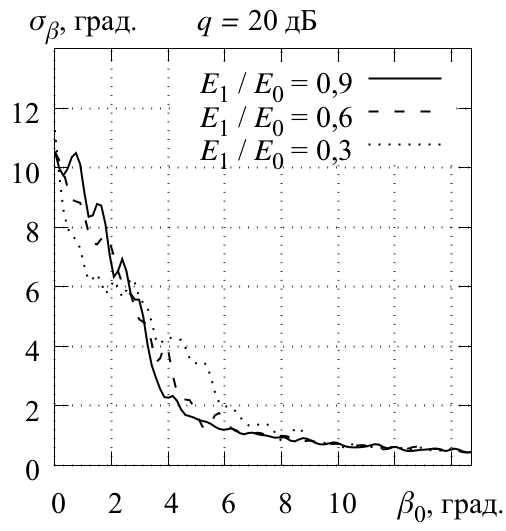
\includegraphics[width=0.33\linewidth]{3/surface/pic2_a}}
  \subfloat[\textit{б)}]{\includegraphics[width=0.33\linewidth]{3/surface/pic2_b}}
  \subfloat[\textit{в)}]{\includegraphics[width=0.33\linewidth]{3/surface/pic2_c}}
  \\
  \subfloat[\textit{г)}]{\includegraphics[width=0.33\linewidth]{3/surface/pic2_d}}
  \subfloat[\textit{д)}]{\includegraphics[width=0.33\linewidth]{3/surface/pic2_e}}
  \subfloat[\textit{е)}]{\includegraphics[width=0.33\linewidth]{3/surface/pic2_f}}

  \caption{Графики угловых зависимостей случайных (\textit{а}, \textit{б}, \textit{в}) и методических (\textit{г}, \textit{д}, \textit{е}) СКО определения угла при различных значениях параметров принятого сигнала: амплитуды (\textit{а}, \textit{г}), угла приема отраженной волны (\textit{б}, \textit{д}) и разности фаз принятых сигналов (\textit{в}, \textit{е}).}
  \label{fig:surface:pic2}
\end{figure}

Возмущения исходных значений сигналов на каждой из антенн производилось путем добавления к ним некоторой случайной величины, распределенной по нормальному закону с нулевым математическим ожиданием и дисперсией, соответствующей заданному ОСШ. Устойчивость предложенного метода определения угла $\beta_0$ оценивалась при значении ОСШ $q = \SI{20}{\deciBells}$. Также при оценке рассматривался идеальный случай, в котором влияние шума пренебрежимо мало, т.е. ОСШ $q = \SI{100}{\deciBells}$. На Рис.~\ref{fig:surface:pic2} приведены графики зависимостей СКО $\sigma_\beta$ от определяемого угла $\beta_0$.

\begin{figure}[hptb]
  \centering
  \subfloat[\textit{а)}]{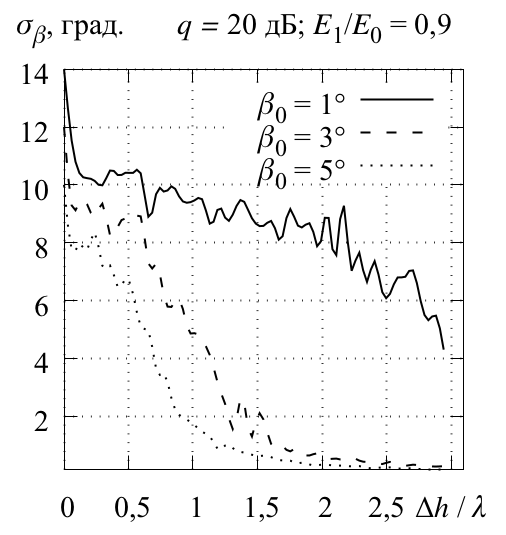
\includegraphics[width=0.33\linewidth]{3/surface/pic3_a}}
  \subfloat[\textit{б)}]{\includegraphics[width=0.33\linewidth]{3/surface/pic3_b}}
  \subfloat[\textit{в)}]{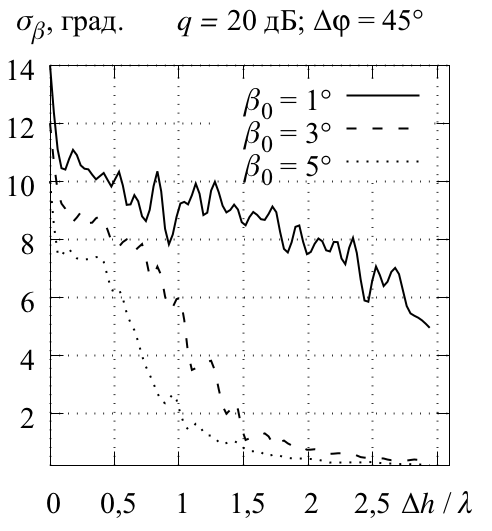
\includegraphics[width=0.33\linewidth]{3/surface/pic3_c}}
  \\
  \subfloat[\textit{г)}]{\includegraphics[width=0.33\linewidth]{3/surface/pic3_d}}
  \subfloat[\textit{д)}]{\includegraphics[width=0.33\linewidth]{3/surface/pic3_e}}
  \subfloat[\textit{е)}]{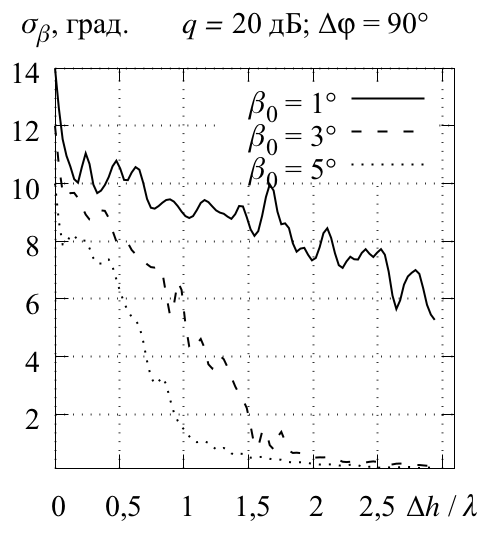
\includegraphics[width=0.33\linewidth]{3/surface/pic3_f}}

  \caption{Графики частотных зависимостей случайных СКО определения угла при различных значениях параметров принятого сигнала: амплитуды (\textit{а}, \textit{г}), угла приема отраженной волны (\textit{б}, \textit{д}) и разности фаз принятых сигналов (\textit{в}, \textit{е}).}
  \label{fig:surface:pic3}
\end{figure}

Также была произведена оценка зависимости СКО от уровня взаимного влияния между антеннами $\Delta h^{}/\lambda$. На Рис.~\ref{fig:surface:pic3} приведены графики этих зависимостей при различных значениях углов $\beta_0$ и значений параметров принятых сигналов.

С помощью моделирования было так же выяснено, что при увеличении ОСШ кривая угловых зависимостей СКО приобретает ярко выраженный L-образный характер, т.е. погрешность резко убывает при определенном значении определяемого угла $\beta_0$. Рис.~\ref{fig:surface:pic4} показывает характер этой зависимости при ОСШ $q = \SI{30}{\deciBells}$.

\begin{figure}[hpbt]
  \centering
  \subfloat[\textit{а)}]{\includegraphics[width=0.33\linewidth]{3/surface/pic4_a}}
  \subfloat[\textit{б)}]{\includegraphics[width=0.33\linewidth]{3/surface/pic4_b}}
  \subfloat[\textit{в)}]{\includegraphics[width=0.33\linewidth]{3/surface/pic4_c}}

  \caption{Графики угловых зависимостей случайных СКО определения угла при различных значениях параметров принятого сигнала: амплитуды (\textit{а}), угла приема отраженной волны (\textit{б}) и разности фаз принятых сигналов (\textit{в})}
  \label{fig:surface:pic4}
\end{figure}

Главное отличие от модели, предложенной в [ВГМНП], состоит в том, что система содержит шесть неизвестных вещественных переменных, а не пять, и поэтому не является переопределенной. Соответственно, нет областей изменения параметров, в которых система несовместна. Сложности, как и следовало ожидать, начинаются при стремлении $\beta_0$ к нулю "--- в этом случае все три коэффициента $u$, $v$ и $c$ уравнения \eqref{eq:u_v_omega_0} становятся малыми, и преобразования, связанные с делением на эти величины, являются неустойчивыми.

Из приведенных в работе графиков среднеквадратичных погрешностей (рис.~\ref{fig:surface:pic2} и~\ref{fig:surface:pic3}) можно сделать следующий вывод: если $\beta_0$ имеет величину порядка $\ang{1}$ "--- $\ang{3}$, то погрешность становится больше самой определяемой величины, т.е. вычисления с практической точки зрения бесполезны. Существенным оказывается и соотношение углов $\beta_0$ и $\beta_1$. С увеличением разности между ними растет и погрешность. Большая разность между этими углами возможна в том случае, когда объект пеленгации находится слишком близко к датчикам. Достаточно важным параметром является разность фаз $\Delta \varphi$ – если пришедшие сигналы приходят в фазе или противофазе, то предложенная модель оказывается неэффективной. Это объясняется тем, что величины $\dot{z}_\text{в}$ и $\dot{z}_\text{н}$ становятся слишком близки друг к другу и критерий разрешимости \eqref{eq:c_good} нарушается для большинства значений $\beta_0$.

\end{document}